\documentclass[tikz,border=6pt]{standalone}
\usepackage[T1]{fontenc}
\usepackage{tikz}
\usetikzlibrary{arrows.meta,positioning,fit}

\begin{document}
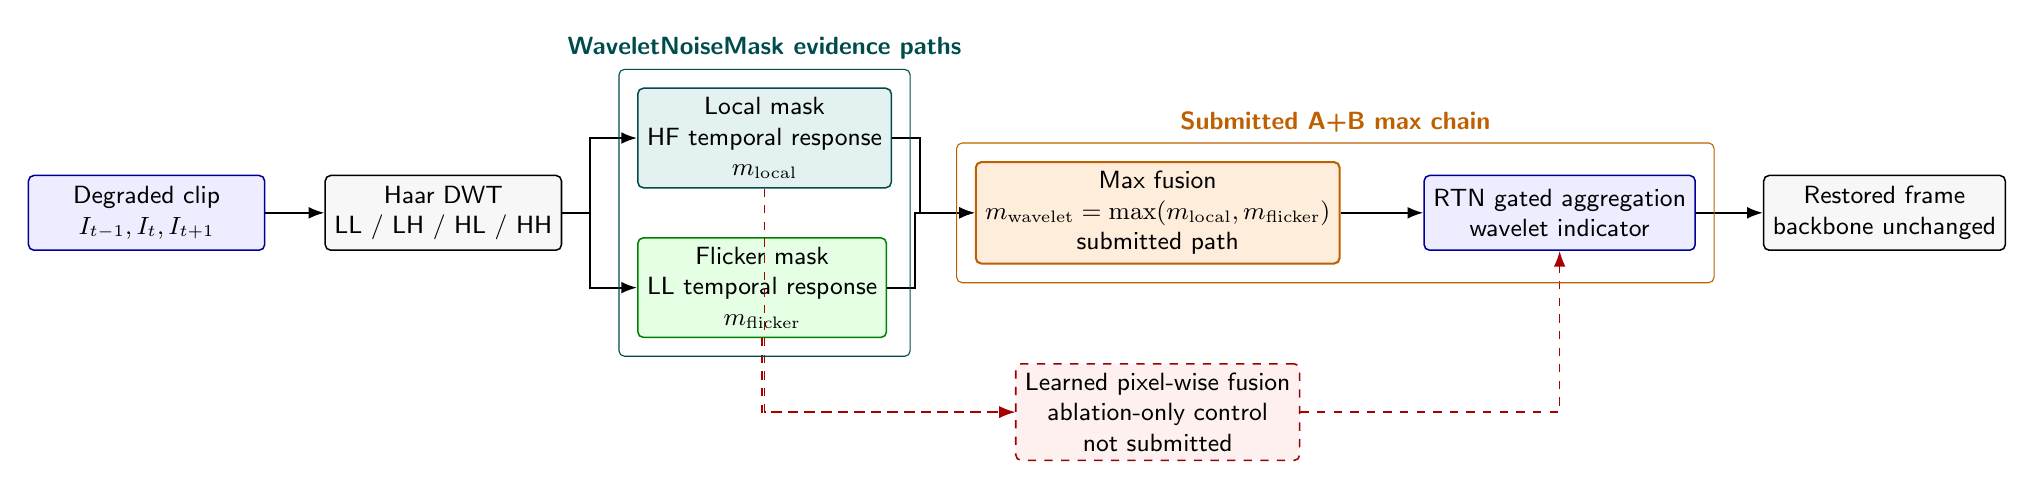
\begin{tikzpicture}[
  font=\sffamily\small,
  box/.style={draw, rounded corners=2pt, align=center, minimum height=0.95cm, minimum width=3.0cm, line width=0.55pt, fill=gray!6},
  input/.style={box, fill=blue!7, draw=blue!60!black},
  local/.style={box, fill=teal!11, draw=teal!60!black},
  flicker/.style={box, fill=green!10, draw=green!50!black},
  fuse/.style={box, fill=orange!14, draw=orange!75!black, line width=0.75pt},
  ablate/.style={box, fill=red!6, draw=red!60!black, dashed},
  arrow/.style={-{Latex[length=2mm]}, line width=0.7pt},
  softarrow/.style={-{Latex[length=2mm]}, line width=0.55pt, dashed}
]

\node[input] (clip) {Degraded clip\\$I_{t-1}, I_t, I_{t+1}$};
\node[box, right=0.75cm of clip] (dwt) {Haar DWT\\LL / LH / HL / HH};

\node[local, right=0.95cm of dwt, yshift=0.95cm] (local) {Local mask\\HF temporal response\\$m_{\mathrm{local}}$};
\node[flicker, right=0.95cm of dwt, yshift=-0.95cm] (flicker) {Flicker mask\\LL temporal response\\$m_{\mathrm{flicker}}$};
\node[fuse, right=1.05cm of local, yshift=-0.95cm] (maxfuse) {Max fusion\\$m_{\mathrm{wavelet}} = \max(m_{\mathrm{local}}, m_{\mathrm{flicker}})$\\submitted path};

\node[input, right=1.05cm of maxfuse] (gate) {RTN gated aggregation\\wavelet indicator};
\node[box, right=0.85cm of gate] (restore) {Restored frame\\backbone unchanged};

\node[ablate, below=1.25cm of maxfuse] (learned) {Learned pixel-wise fusion\\ablation-only control\\not submitted};

\draw[arrow] (clip) -- (dwt);
\draw[arrow] (dwt.east) -- ++(0.35,0) |- (local.west);
\draw[arrow] (dwt.east) -- ++(0.35,0) |- (flicker.west);
\draw[arrow] (local.east) -- ++(0.35,0) |- (maxfuse.west);
\draw[arrow] (flicker.east) -- ++(0.35,0) |- (maxfuse.west);
\draw[arrow] (maxfuse) -- (gate);
\draw[arrow] (gate) -- (restore);

\draw[softarrow, red!65!black] (local.south) |- (learned.west);
\draw[softarrow, red!65!black] (flicker.south) |- (learned.west);
\draw[softarrow, red!65!black] (learned.east) -| (gate.south);

\node[draw=teal!60!black, rounded corners=2pt, inner sep=0.23cm, fit=(local) (flicker), label={[font=\sffamily\bfseries\small, text=teal!60!black]above:WaveletNoiseMask evidence paths}] {};
\node[draw=orange!75!black, rounded corners=2pt, inner sep=0.23cm, fit=(maxfuse) (gate), label={[font=\sffamily\bfseries\small, text=orange!75!black]above:Submitted A+B max chain}] {};

\end{tikzpicture}
\end{document}
